% Benvenuti nel template per le relazioni di Sperimentazioni di Fisica 1 del corso triennale in Astronomia dell'Università di Padova.
% Per compilarlo, cliccate su Menu, selezionate come compilatore "pdfLaTeX", TeX Live Version 2020 (o uno degli altri, whatever works), e come documento principale "Relazione.tex"

%%% Preambolo del documento %%%
% Non toccate questa roba, a meno che non siate abbastanza sgamati da sapere quello che state facendo, tipo vi piacciono di più certi pacchetti rispetto ad altri, o magari ve ne manca qualcuno.
\documentclass[a4paper, titlepage]{article}
\usepackage[T1]{fontenc}
\usepackage[utf8]{inputenc}
\usepackage[italian]{babel}
\usepackage{amsmath}
\usepackage{listings}
\usepackage{textcomp}
\usepackage{multirow}
\usepackage{multicol}
\usepackage{booktabs}
\usepackage{graphicx}
\usepackage{floatflt}
\usepackage{epsfig}
\usepackage{pstricks}
\usepackage{subfigure}
\usepackage[labelfont=bf, font=scriptsize]{caption}
\usepackage[italian]{varioref}
\usepackage[suftesi]{frontespizio}
\usepackage{color}
\usepackage{tikz}
\usepackage{caption}
\usepackage{pgfplots}
\usepackage{comment}
\usepackage{lipsum}
\pgfplotsset{compat=1.16}

%%% Il documento vero e proprio %%%
\begin{document}

%%% Frontespizio %%%
% Questa serie di comandi genera il frontespizio della relazione.
% Cambiate: l'Anno Accademico, Data e Titolo della relazione, il nome degli appartenenti al gruppo con annessa matricola e mail istituzionale. Se siete due o quattro in gruppo, basta togliere/inserire una riga Candidato.
% NON toccate i comandi con accanto con CTT (Can't Touch This).
% !!! NOTA PER LA CORRETTA VISUALIZZAZIONE DEL FRONTESPIZIO. !!!
% Quando si compila un file su Overleaf, per velocizzare le successive compilazioni questi genera una cache, e da questa prende gli elementi che, a senso suo, non sono cambiati nel testo. Quindi per quanto vi possiate ostinare a compilare, vedrete sempre il primo frontespizio che ha compilato (quello con NomeCognome etc etc) e non le ultime modifica.
% Come evitare ciò, e visualizzare il frontespizio con i vostri nomi, cognomi e numeri matricola? Così: cliccate sull'icona accanto a Recompile, quella con il simbolo del documento, e successivamente sul simbolo del cestino (Clear cached files). Liberate la cache, modificate il frontespizio, e ricompilate. Così dovreste riuscire a vedere nel file compilato le vostre modifiche al frontespizio. Ricordatevi di svuotare la cache del file Overleaf ogni volta che volete modificare qualcosa nel frontespizio.
\begin{frontespizio}
\Universita{Padova} % CTT
\Logo{Figure/logo_unipd} % CTT
\Divisione{Esercitazioni SPICE} % CTT
\Corso[Laurea Triennale]{Ingegneria Informatica} % CTT, a meno che non cambi la denominazione del corso
\Annoaccademico{2022-2023}
\Titoletto{Relazione Prima Esercitazione SPICE} % CTT
\Titolo{Prima Esercitazione SPICE}
\Sottotitolo{05/12/2022}
\NCandidati{Studente} % CTT
\Candidato[2052644]{Filippo Stella, \textsf {filippo.stella.1@studenti.unipd.it}}
\NRelatore{Docente}{} % CTT
\Relatore{Prof. Enrico Zanoni} % CTT, a meno che non sia cambiato il Prof.
\end{frontespizio}
\IfFileExists{\jobname-frn.pdf}{}{%
\immediate\write18{pdflatex \jobname-frn}} % ASSOLUTAMENTE CTT, è il comando che materialmente vi genera il frontespizio.

%%% Indice %%%
\tableofcontents

\newpage
%%% Sezioni %%%
% Qui inizia la relazione vera e propria.
% Le Sezioni sono singoli file .tex dentro la cartella Sezioni. Potete a libera scelta scrivere tutto su un singolo file e chiamare all'interno di questi con il comando \section{} le varie sezioni, oppure dividere le singole sezioni in più file Sezione_i.tex, e poi inserirle tutte con \input{Sezioni/Sezione_i.tex} per i = 1 ... N
% Titolo della sezione e label. Vi consiglio, per questioni di ordine mentale e rapidità successiva di reference, di etichettare le label in modo sensato, con riferimento chiaro a cosa si sta etichettando. Quindi sec:nomesezione per una sezione, im:nomeimmagine per una immagine, e via dicendo.
\section{Primo Esercizio}\label{sec:primoEsercizio} 
Amplificatore Audio per Auricolari
\begin{figure}[h]
    \centering
    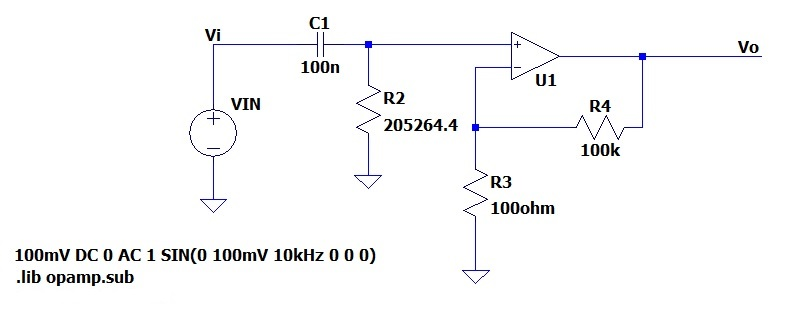
\includegraphics[width=0.9\textwidth]{Figure/Circuito1.jpg}
    \caption{Circuito del primo esercizio}
    \label{fig:Circuito1}
\end{figure}\\
Listato SPICE della rete considerata:\\
\\
C1 N001 Vi 100n\\
R2 N001 0 205264.4\\
R3 N002 0 100\\
R4 Vo N002 100k\\
XU1 N002 N001 Vo opamp Aol=100K GBW=10Meg\\
VIN Vi 0 100mV DC 0 AC 1 SIN(0 100mV 10kHz 0 0 0)\\
.ac dec 10 1 1MEG\\
.lib opamp.sub\\
.backanno\\
.end\\
\subsection{Analisi Analitica}\label{subsec:analisiAnalitica}
Si procede considerando l'amplificatore ideale
\begin{itemize}
\item 
    \begin{equation}\label{eq:eqMorsettiAmplificatore}
    V_{-} = V_{+} = V_{i} \dfrac{R_{2}}{R_{2} + \dfrac{1}{sC_{2}}} = V_{i} \dfrac{sR_{2}C_{2}}{1 + sC_{2}R_{2}}
    \end{equation}
\item 
    \begin{equation}\label{eq:eqCorrenteR3}
    I_{R_{3}} = \dfrac{V_{-}}{R_{3}} = V_{i} \dfrac{sR_{2}C_{2}}{R_{3} (1 + sC_{2}R_{2})}
    \end{equation}
\item
    \begin{equation}\label{eq:eqTensioneUscita1}
    V_{o} = I_{4} R_{4} + V_{-} = V_{i} ( \dfrac{R_{4}}{R_{3}} \dfrac{sR_{2}C_{2}}{1 + sC_{2}R_{2}} + \dfrac{sR_{2}C_{2}}{1 + sC_{2}R_{2}} )
    \end{equation}
    \begin{equation}\label{eq:eqTensioneUscita2}
    V_{o} = V_{i} ( \dfrac{sR_{2}C_{2} (R_{3}+R_{4})}{R_{3}} \dfrac{1}{1 + sC_{2}R_{2}}  )
    \end{equation}
\end{itemize}
La risposta in frequenza del circuito considerato presenta uno zero nell'origine e un polo ad una frequenza f.
\begin{itemize}
\item 
    Guadagno \begin{equation}\label{eq:eqGuadagno}
    K = \dfrac{R_{2}C_{2} (R_{3}+R_{4})}{R_{3}} = 20,547
    \end{equation}
    \begin{equation}\label{eq:eqGuadagnoDecibel}
    (K)_{dB} = 20 log_{10} (K) = 26,25\hspace{2pt}dB
    \end{equation}
\item 
    La risposta presenta uno zero nell'origine
    \begin{equation}\label{eq:eqPoloOrigine}
    +20 \hspace{2pt}\dfrac{dB}{DEC}
    \end{equation}
\item
    La risposta presenta un polo alla frequenza di taglio
    \begin{equation}\label{eq:eqPulsazioneTaglio}
    \omega = \dfrac{1}{R_{2}C_{2}} = 48,71
    \end{equation}
    \begin{equation}\label{eq:eqFrequenzaTaglio}
    f = \dfrac{\omega}{2\pi} = 7,75\hspace{2pt}Hz
    \end{equation}
\end{itemize}

\subsection{Frequenza di Taglio Inferiore}\label{subsec:frequenza_taglio_inferiore}
Come calcolato precedentemente la risposta in frequenza presenta un polo alla frequenza di taglio  (Equazione n° \ref{eq:eqFrequenzaTaglio})
$$f = \dfrac{\omega}{2\pi} = 7,75\hspace{2pt}Hz$$

\subsection{Diagramma di Bode}\label{subsec:diagramma_bode}
Il diagramma di Bode che risulta dall'analisi analitica è il seguente\\
\begin{figure}[h]
    \centering
    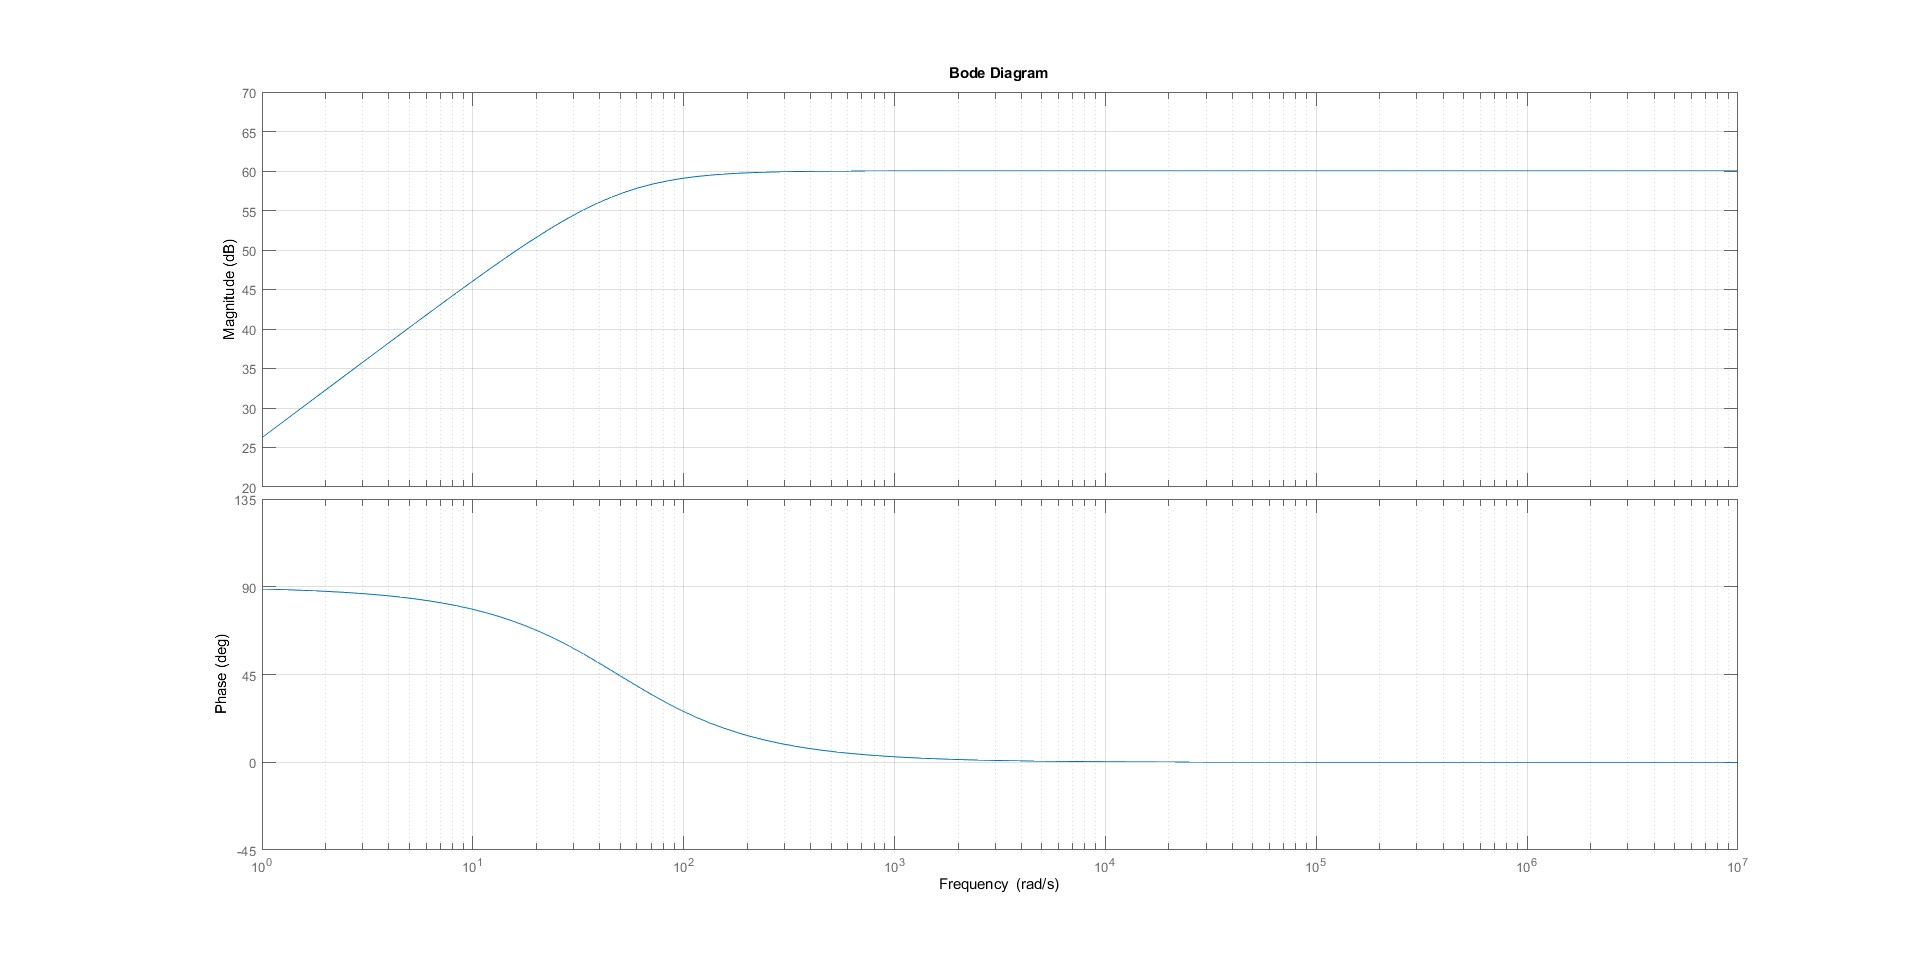
\includegraphics[width=1\textwidth]{Figure/BodeAnalitico.jpg}
    \caption{Diagramma di Bode ottenuto dall'analisi analitica}
    \label{fig:bodeAnalitico}
\end{figure}
\newpage
\subsection{Simulazione SPICE}\label{subsec:simulazione_spice}
Simulando su SPICE il circuito otteniamo il seguente diagramma di Bode.\\
\begin{figure}[h]
    \centering
    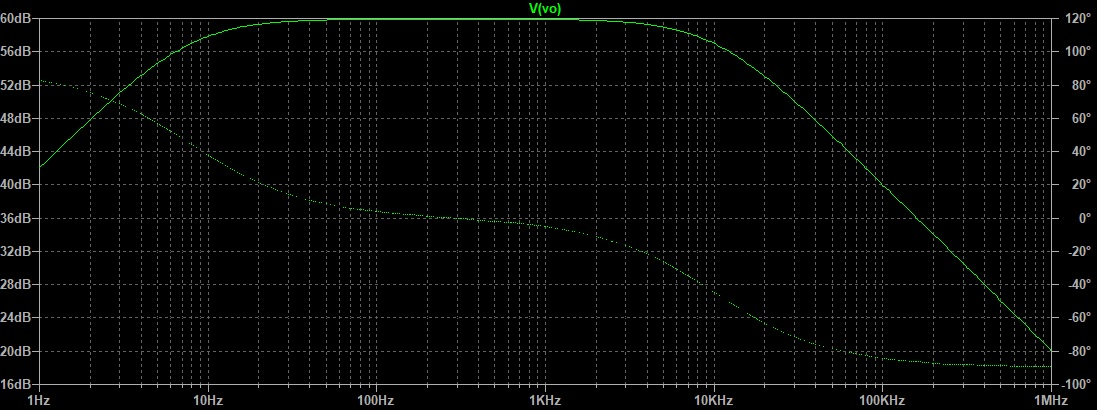
\includegraphics[width=1\textwidth]{Figure/Bode 1.4_1.jpg}
    \caption{Grafico di Bode non ideale}
    \label{fig:bode_non_ideale}
\end{figure}\\
Il precedente diagramma differisce da quello calcolato, in quanto l'amplificatore operazionale utilizzato da SPICE non è un amplificatore ideale.\\
Per avere condizioni simili a quelle di un amplificatore ideale dobbiamo incrementare il rapporto guadagno x larghezza di banda. Dopo aver incrementato il rapporto di un fattore 1000 infatti la simulazione produce il seguente grafico.\\
\begin{figure}[h]
    \centering
    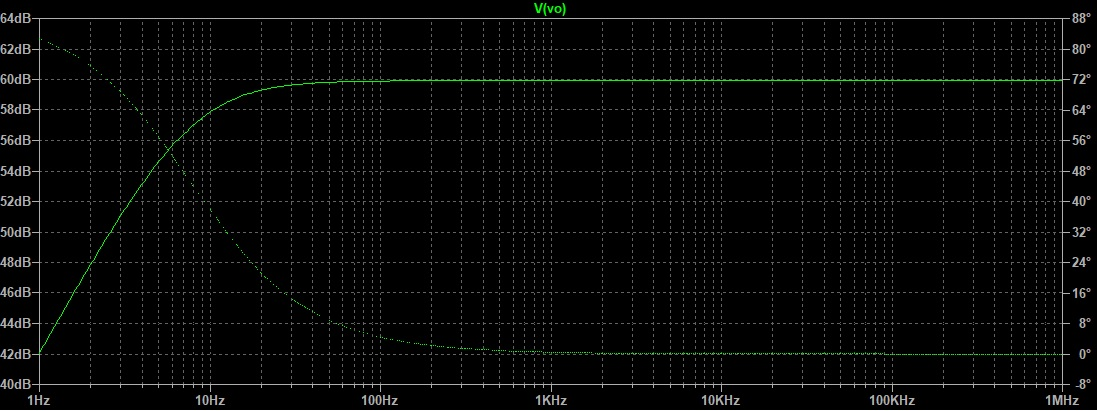
\includegraphics[width=1\textwidth]{Figure/Bode 1.4_2.jpg}
    \caption{Grafico di Bode ideale}
    \label{fig:bode_ideale}
\end{figure}\\

\subsection{Aumentare la Banda}\label{subsec:aumentare_banda}
Per aumentare la banda dell'amplificatore potremmo ridurre il guadagno.

\newpage
\subsection{Simulazione SPICE per Amplificatore LT1115}\label{subsec:simulazione_LT1115}
Si considera ora una variante del circuito, sostituendo l'amplificatore operazionale ideale con un amplificatore reale LT1115.
\begin{figure}[h]
    \centering
    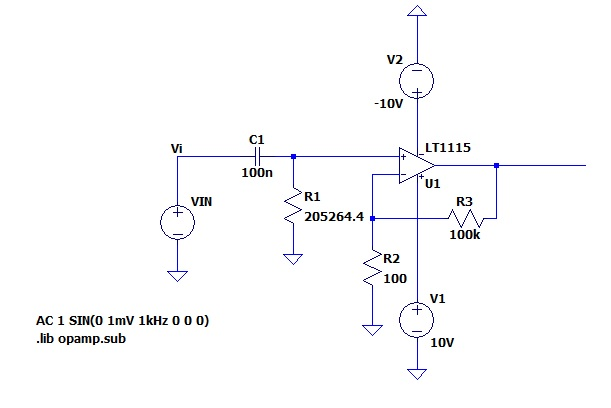
\includegraphics[width=0.9\textwidth]{Figure/Circuito.jpg}
    \caption{Variante circuito del primo esercizio}
    \label{fig:Circuito}
\end{figure}\\
Listato SPICE della rete considerata:\\
\\
C1 N002 Vi 100n\\
R1 N002 0 205264.4\\
R2 N004 0 100\\
R3 N003 N004 100k\\
V1 N005 0 10V\\
V2 N001 0 -10V\\
VIN Vi 0 AC 1 SIN(0 1mV 1kHz 0 0 0)\\
XU1 N002 N004 N005 N001 N003 LT1115\\
.tran 5m\\
.lib opamp.sub\\
.lib LTC.lib\\
.backanno\\
.end\\
\\
Alimentando il circuito con un generatore di tensione sinusoidale con ampiezza 1 mV e frequenza 1 KHz si ottiene la seguente forma d'onda in uscita dall'amplificatore.
\newpage
\begin{figure}[h]
    \centering
    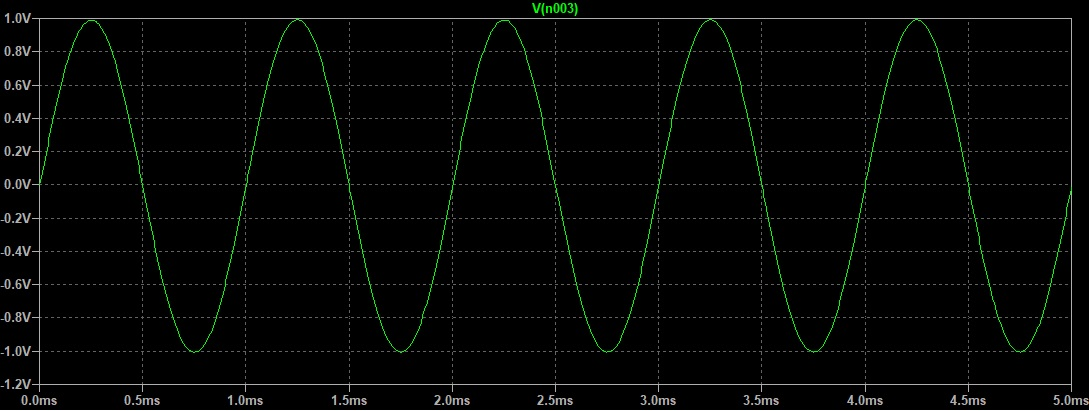
\includegraphics[width=1\textwidth]{Figure/Uscita 1.6.jpg}
    \caption{Forma d'onda in uscita dall'amplificatore per parametri di 1 mV e 1 KHz}
    \label{fig:UscitaCircuito}
\end{figure}

\subsection{Diagramma di Bode}\label{subsec:diagramma_bode_variante}
Simulando con SPICE il circuito per frequenze da 1 Hz a 1 MHz si ottiene il seguente diagramma di Bode.
\begin{figure}[h]
    \centering
    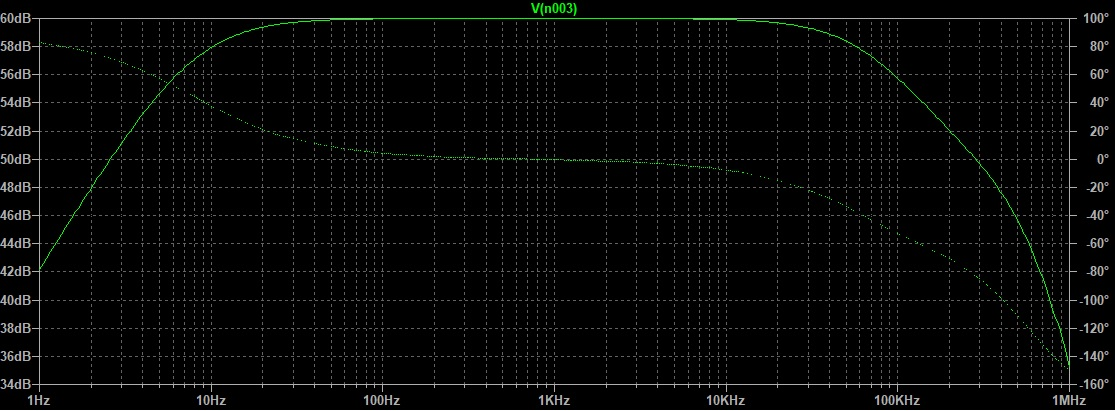
\includegraphics[width=1\textwidth]{Figure/Bode 1.7.jpg}
    \caption{Grafico di Bode per amplificatore LT1115 da 1 Hz a 1 MHz}
    \label{fig:bode_lt1115}
\end{figure}

\newpage
\subsection{Tensione di Saturazione}\label{subsec:saturazione}
Simulando varie ampiezze di ingresso con SPICE otteniamo il seguente risultato\\
\begin{figure}[h]
    \centering
    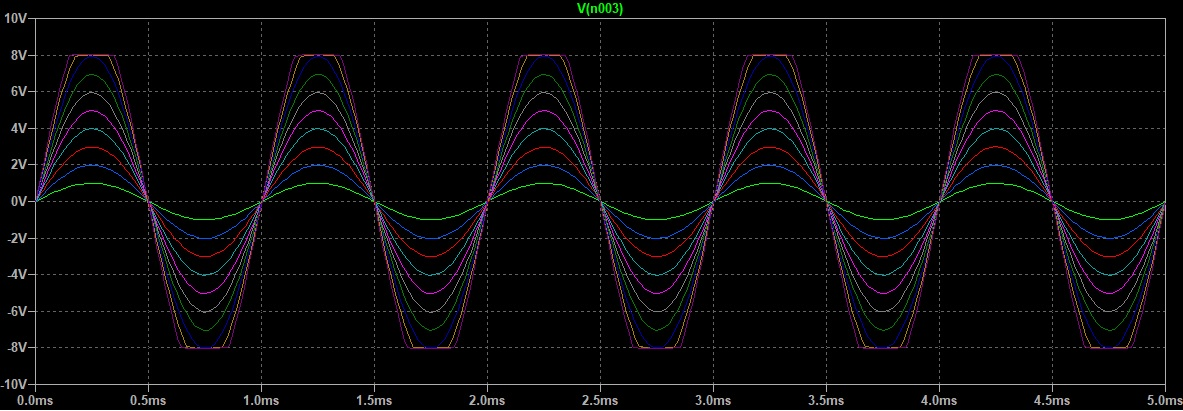
\includegraphics[width=1\textwidth]{Figure/SaturazioneAnalisi 1.8.1.jpg}
    \caption{Forme d'onda in uscita per varie ampiezze in ingresso}
    \label{fig:saturazione_analisi}
\end{figure}\\
Osservando il grafico possiamo notare che la tensione di saturazione per l'amplificatore LT1115 è di 8 V
\newline
Fissiamo ora la frequenza del generatore a 1KHz e calcoliamo analiticamente l'ampiezza di ingresso per la quale l'amplificatore satura.\\
$$s = j\omega$$ $$\omega = 2\pi * f$$
\begin{equation}\label{eq:eqAmpiezzaSaturazione}
V_{o} = V_{i}\dfrac{\dfrac{j\omega R_{2}C_{2}(R_{3}+R_{4})}{R_{3}}}{1+j\omega C_{2}R_{2}} = V_{i}\dfrac{j\omega20,55}{1 + j\omega0,0205} = V_{i}\dfrac{j441100\pi}{1 + j41\pi}
\end{equation}
\begin{equation}\label{eq:eqAmpiezzaSaturazioneModuli}
|V_{o}| = |V_{i}| * \big| \dfrac{j441100\pi}{1 + j41\pi} \big|
\end{equation}
\begin{equation}\label{eq:eqAmpiezzaSaturazioneRisultato}
|V_{i}| < \dfrac{8}{1002,39} = 8\hspace{2pt}mV
\end{equation}
Come trovato nell'equazione \ref{eq:eqAmpiezzaSaturazioneRisultato} l'ampiezza in ingresso per la quale l'amplificatore satura è 8 mV.\\
Simulando ora il circuito con un'ampiezza di ingresso di 16 mV otteniamo il seguente risultato
\begin{figure}[h]
    \centering
    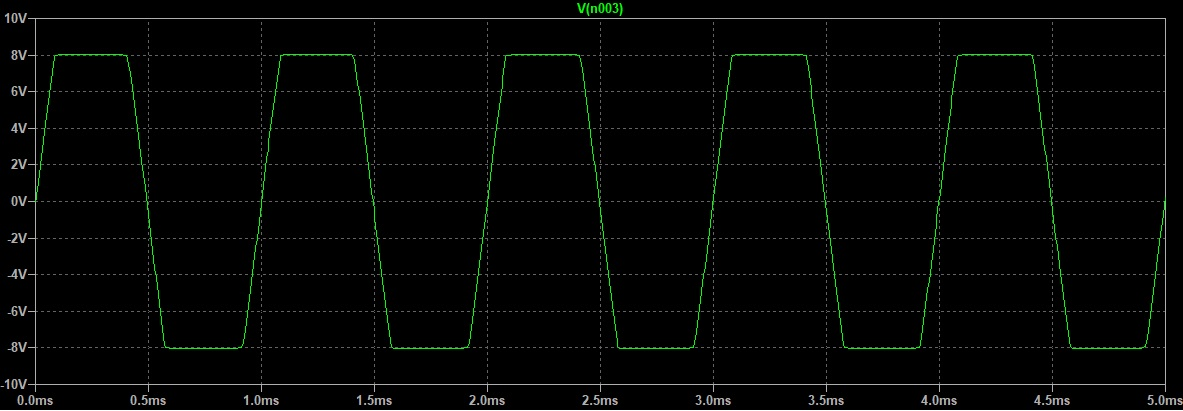
\includegraphics[width=1\textwidth]{Figure/SaturazioneUscita 1.8.2.jpg}
    \caption{Forme d'onda in uscita per un ampiezza di 16 mV}
    \label{fig:saturazione_uscita}
\end{figure}\\	
\newpage
\section{Secondo Esercizio}\label{Sec:SecondoEsercizio}
Sensore Resistometrico
\begin{figure}[h]
    \centering
    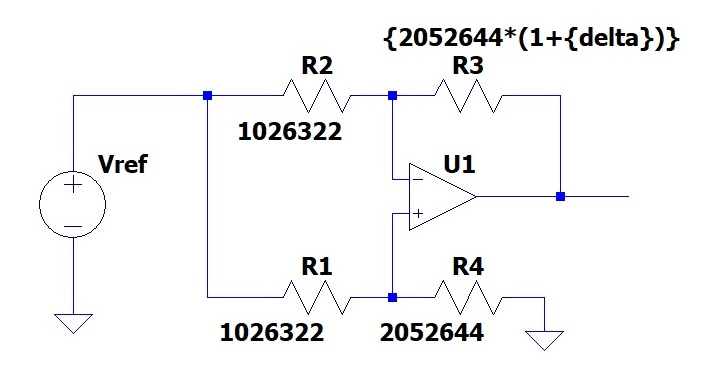
\includegraphics[width=0.9\textwidth]{Figure/Circuito2.jpg}
    \caption{Circuito del secondo esercizio}
    \label{fig:Circuito2}
\end{figure}\\
Listato SPICE della rete considerata:\\
\\
XU1 N002 N004 N003 opamp Aol=100K GBW=10Meg\\
R1 N004 N001 1026322\\
R2 N002 N001 1026322\\
R3 N003 N002 {2052644*(1+{delta})}\\
R4 0 N004 2052644\\
Vref N001 0\\
.inc opamp.sub\\
.step param delta 0 1 0.1\\
.dc Vref 0 -18.75 0.5\\
.backanno\\
.end\\

\subsection{Analisi Analitica}\label{subsec:analisiAnaliticaSecondo}
Per una Vref generica cerchiamo la relazione tra ingresso e uscita del circuito
\begin{itemize}
\item 
    \begin{equation}\label{eq:eqMorsettiAmplificatoreSecondo}
    V_{-} = V_{+} = V_{ref} \dfrac{R}{R_{1} + R}
    \end{equation}
\item 
    \begin{equation}\label{eq:eqCorrenteRSecondo}
    I_{R_{1+\delta}} = \dfrac{V_{-} - V_{ref}}{R_{1}} = \dfrac{V_{ref}}{R_{1}} ( \dfrac{R}{R_{1} + R} - 1 )
    \end{equation}
\item
    \begin{equation}\label{eq:eqTensioneUscitaSecondo1}
    V_{out} = I_{R(1+\delta)} R(1+\delta) + V_{-}
    \end{equation}
    \begin{equation}\label{eq:eqTensioneUscitaSecondo2}
    V_{out} = V_{ref} \dfrac{R(1+\delta)}{R_{1}}(\dfrac{R}{R_{1} + R} - 1) + V_{ref} \dfrac{R}{R_{1} + R}
    \end{equation}
    \begin{equation}\label{eq:eqTensioneUscitaSecondo3}
    V_{out} = V_{ref} (\dfrac{-R_{1}}{R_{1} + R} \dfrac{R(1+\delta)}{R_{1}} + \dfrac{R}{R_{1} + R})  
    \end{equation}
    \begin{equation}\label{eq:eqTensioneUscitaSecondo4}
    V_{out} = V_{ref} (-\dfrac{R}{R_{1} + R} -\dfrac{R\delta}{R_{1} + R} + \dfrac{R}{R_{1} + R}) = - V_{ref} \dfrac{R}{R_{1} + R} \delta 
    \end{equation}
\end{itemize}

\subsection{Dimensionamento del Circuito}\label{subsec:dimensionamentoCircuito}
Come trovato nella formula \ref{eq:eqTensioneUscitaSecondo4} la relazione tra tensione di uscita e tensione di ingresso è la seguente $$V_{out} = - V_{ref} \dfrac{R}{R_{1} + R} \delta$$
Andiamo ora a dimensionare il circuito in modo che $$V_{out} = 12,5 \delta$$
Fissiamo le resistenze
$$R = 2052644$$
$$R_{1} = \dfrac{R}{2} = 1026322$$
Ricaviamo quindi la tensione del generatore in ingresso
\begin{equation}\label{eq:eqTensioneIngresso}
V_{ref} = -12,5\dfrac{R_{1} + R}{R} = -12,5\dfrac{3}{2} = -18,75 V
\end{equation}

\subsection{Corrente attraverso Sensore Resistometrico}\label{subsec:correnteSensoreResistometrico}
Simulando con SPICE il circuito e facendo variare la tensione in ingresso e il parametro variabile del sensore resistometrico otteniamo il seguente grafico per la corrente che scorre nella resistenza.
\begin{figure}[h]
    \centering
    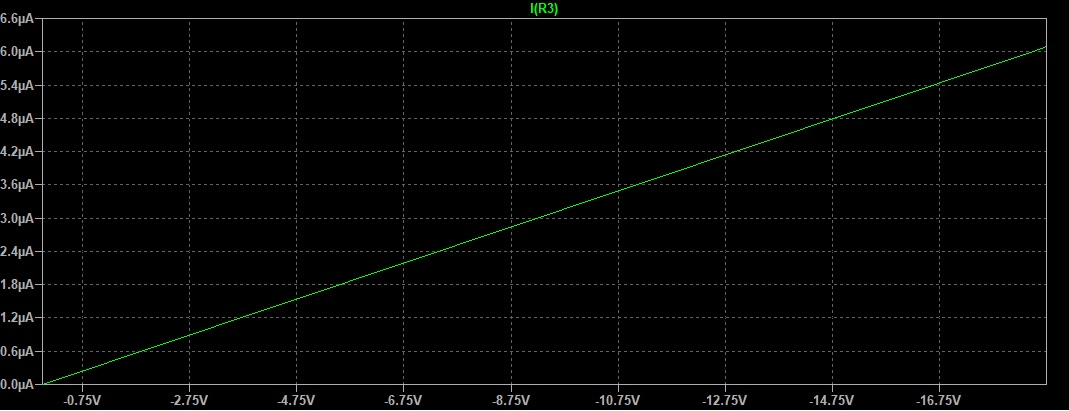
\includegraphics[width=1\textwidth]{Figure/UscitaCorrente.jpg}
    \caption{Corrente che attraversa il sensore resistometrico}
    \label{fig:correnteSensoreResistometrico}
\end{figure}


\newpage
%%% Appendici %%%
% Eventuali appendici vanno qui. Se non avete appendici da inserire, togliete/commentate queste righe.
%\appendix
%\section{Appendice A}\label{app:Appendice A}
\lipsum	

\end{document}

% Credits: basato sulle relazioni di laboratorio di Nicola Bellucco, Marco Codato e Erica Korb.